
\documentclass[xcolor=dvipsnames]{beamer} % dvipsnames gives more built-in colors
\usepackage[utf8]{inputenc}
\usepackage[spanish]{babel}

\mode<presentation> {

\usetheme{CambridgeUS}

%\setbeamertemplate{footline} % To remove the footer line in all slides uncomment this line
\setbeamertemplate{footline}[page number] % To replace the footer line in all slides with a simple slide count uncomment this line

\setbeamertemplate{navigation symbols}{} % To remove the navigation symbols from

\definecolor{utfsmred}{HTML}{D60019}
\definecolor{utfsmyellow}{HTML}{F7AE00}
\definecolor{utfsmgreen}{HTML}{008452}
\definecolor{utfsmblue}{HTML}{004B85}


\newenvironment<>{rosa}[1][]{
  \setbeamercolor{block title example}{fg=white,bg=blue!75!black}%
  \begin{example}#2[#1]}{
  \end{example}
}



\usecolortheme[named=utfsmblue]{structure}
\setbeamercolor{titlelike}{parent=structure,fg=utfsmblue}
\setbeamercolor{frametitle}{fg=utfsmblue}

%\setbeamercolor{section in head/foot}{bg=Brown}
%\setbeamercolor{author in head/foot}{bg=Brown}
%\setbeamercolor{date in head/foot}{fg=Brown}

\setbeamercolor*{enumerate item}{fg=utfsmred}
\setbeamercolor*{enumerate subitem}{fg=utfsmred}
\setbeamercolor*{enumerate subsubitem}{fg=utfsmred}

\setbeamercolor*{itemize item}{fg=utfsmred}
\setbeamercolor*{itemize subitem}{fg=utfsmred}
\setbeamercolor*{itemize subsubitem}{fg=utfsmred}

\setbeamercolor{item projected}{bg=utfsmred}


\setbeamertemplate{itemize items}[square]
\setbeamertemplate{enumerate items}[default]


\setbeamercolor{section in head/foot}{bg=utfsmblue}

\setbeamercolor{block title}{bg=utfsmblue!80,fg=white}
\setbeamercolor{block title alerted}{bg=utfsmred!80,fg=white}
\setbeamercolor{block title example}{bg=utfsmgreen!80,fg=white}

\setbeamertemplate{sections/subsections in toc}[square]
\setbeamercolor{section number projected}{bg=utfsmblue,fg=white}


}

\usepackage{graphicx} % Allows including images
\usepackage{booktabs} % Allows the use of \toprule, \midrule and \bottomrule in tables

\usepackage{listings}
\lstset{ %
language=bash,
basicstyle=\normalsize\ttfamily,
keywordstyle=,
numbers=none,
numberstyle=\tiny\ttfamily,
stepnumber=1,
showspaces=false,
showstringspaces=false,
showtabs=false,
breaklines=true,
frame=tb,
framerule=0.5pt,
tabsize=4,
framexleftmargin=0.5em,
framexrightmargin=0.5em,
xleftmargin=0.5em,
xrightmargin=0.5em,
}

%----------------------------------------------------------------------------------------
%	TITLE PAGE
%----------------------------------------------------------------------------------------

\title{Cap.0. Presentación del curso}
\subtitle{\small{Seminario de Desarrollo de Software - Casa Central.}}
\author{Maximiliano Osorio\\\small{mosorio@inf.utfsm.cl}} 
\institute[UTFSM]
{
Universidad Técnica Federico Santa María
\medskip
}
\date{\today} % Date, can be changed to a custom date

\begin{document}

\maketitle
\section{Maximiliano}
%------------------------------------------------

\section{Asignatura}
%------------------------------------------------
\begin{frame}[fragile]
\frametitle{Descripción}
La asignatura busca...
\begin{itemize}
	\item  \ldots desarrollar y potenciar habilidades del estudiante
	\item  \ldots de acuerdo a los perfiles requeridos en ámbito profesional 
	\item  \ldots focalizándose en el área de operaciones específicamente el proceso de despliegue de la solución.
\end{itemize}
\end{frame}

\section{Origen}


\begin{frame}[fragile]
\frametitle{¿Cómo nace este curso?}
Nace al observar problemas y oportunidades.
\end{frame}




\frame{
\frametitle{DevOps}
  \begin{figure}
   \includegraphics[scale=0.45]{../img/Devops.png}
   \caption{Devops \footnote{Fuente: \url{https://en.wikipedia.org/wiki/DevOps} }}
  \end{figure}
}


\begin{frame}[fragile]
\frametitle{DevOps}

\begin{itemize}
  \item Devs, QA y sysadmin trabajan de forma más unida en comparación a ambientes tradicionales.
  \item Desde el desarrollo ágil, las aplicaciones comenzaron a desarrollarse de manera muy rápida en un proceso iterativo.
  \item Fallar, arreglar, fallar, arreglar.

\end{itemize}

\end{frame}


\begin{frame}[fragile]
\frametitle{}
\begin{figure}
\centering

\includegraphics[width=\textwidth,height=1\textheight,keepaspectratio]{images/m1}
\end{figure}

\end{frame}



\begin{frame}[fragile]
\frametitle{DevOps}

\begin{itemize}

  \item Las metodologias ágiles unieron las áreas, causando que sysadmin y otros profesionales unieran sus habilidades \ldots
  \item \ldots \textbf{encontrar errores} de aplicaciones y reparar problemas de códigos.
\end{itemize}

\end{frame}

%------------------------------------------------


%------------------------------------------------

\begin{frame}[fragile]
\frametitle{Equipo}

\begin{itemize}
  \item Muchos (libros y personas) hablan que un buen flujo de comunicación entre Dev y Ops es crucial para establecer una fundación solida.
  \item Sitios modernos cada vez tiene más capas complejas que quieren diferentes habilidades.
\end{itemize}

\end{frame}
%------------------------------------------------

\begin{frame}[fragile]
\frametitle{}
\begin{itemize}
  \item Al parecer ser un buen dev no es suficiente, ser un buen ops no es suficiente.
 \pause
  \item Devs y operaciones deben trabajar al mismo nivel, sin \textbf{pasarse la pelota} a otro para complementar las tareas necesarios.

\end{itemize}

\end{frame}
%------------------------------------------------

\begin{frame}[fragile]
\frametitle{¿Qué debo aprender?}

Devs
\begin{itemize}
  \item Operating systems
  \item Network architecture
  \item Network security
  \item Web application security
  \item Configuration management
  \item Automation practices
\end{itemize}


\end{frame}
%------------------------------------------------

\begin{frame}[fragile]
\frametitle{¿Qué debo aprender?}

Ops
\begin{itemize}
  \item Communications
  \item Configuration management
  \item Programming	
  \item Software design and architecture
\end{itemize}


\end{frame}
%------------------------------------------------

\subsection{Ofertas de empleo}

\frame{ 
\frametitle{Ejemplo} 

 \begin{itemize}
\item Backend Software Engineer: Es deseable y sumas puntos si has desarrollado y mantenido aplicaciones en AWS
\pause
\item Desarrollador Full-Stack Django: Ojalá que tengas conocimiento de Vagrant, Docker, u otro software de abstracción de plataformas.
 \pause

\item DevOps / QA: Proponer e implementar mejoras en la infraestructura a modo de garantizar el buen funcionamiento de los sistemas actuales.


 \end{itemize}


}



\begin{frame}[fragile]
\frametitle{Ejemplo}
\begin{itemize}
	\item DevOps: Linux/VPS: HAproxy, Varnish, Squid, Docker, Iptables, Deis (Cluster), Jenkins.
	\item Ingeniero DevOps: Sólidos conocimientos de programación procedural, orientada a objetos y bases de datos relacionales.
	\item Experiencia desplegando y configurando PostgreSQL, Memcache, Redis,...
	\item Ingeniero Desarrollo Python: También deberá contar con conocimientos avanzados de comandos básicos Unix/Linux.
\end{itemize}

\end{frame}


\begin{frame}[fragile]
\frametitle{}
\begin{figure}
\centering

\includegraphics[width=\textwidth,height=1\textheight,keepaspectratio]{images/m2}
\end{figure}


\end{frame}

	
\section{Curso}
\begin{frame}[fragile]
\frametitle{¿De qué se trata de este curso?}

Este curso se trata de:
\begin{itemize}
  \item Curso práctico
  \item Para despliegue de plataformas web
  \item Aportar conocimientos del área del lado de operaciones
  
\end{itemize}

\end{frame}
%------------------------------------------------
\begin{frame}[fragile]
\frametitle{Contenidos}

\begin{itemize}
  \item Conocimientos básicos de UNIX
  \item Buenas prácticas en sistemas Linux.
  \item Buenas prácticas de seguridad
  \item Configuración de base de datos
  \item Balanceo de carga
  \item Automatización (Configuration management)
  \item Optimizaciones para web server y sistemas de caching
\end{itemize}


\end{frame}
%------------------------------------------------



\begin{frame}[fragile]
\frametitle{Metodología de clase}
\begin{itemize}
  \item Clases expositivas sobre contenidos para afrontar el laboratorio.
  \item Clases de consultas sobre el laboratorio.
\end{itemize}

\end{frame}
%------------------------------------------------

\begin{frame}[fragile]
\frametitle{Evaluación}

La nota final del estudiante será calculada con el promedio de quices (PQ) y el promedio de laboratorio (PL)\\
\begin{equation}
NF = 0.2 \cdot PQ + 0.8 \cdot PL
\end{equation}

\end{frame}
%------------------------------------------------

\begin{frame}[fragile]
\frametitle{Fechas de laboratorios}
\begin{itemize}
  \item Laboratorio \#1: Configuración básica de la infraestructura \\ 
11 de septiembre al 24 de septiembre \\
	\item Laboratorio \#2: Instalación del software y componentes \\
2 de octubre al 15 de octubre \\

\item Laboratorio \#3: Motor de base de datos \\
23 de octubre al 5 de noviembre \\

\item Laboratorio \#4: Balanceo de carga y automatización \\
3 de noviembre al 26 de noviembre \\

\item Laboratorio \#5: Caching y pruebas de carga \\
4 de diciembre al 17 de diciembre \\
\end{itemize}
\end{frame}
%------------------------------------------------

\begin{frame}[fragile]
\frametitle{Fechas quices }
\begin{itemize}
  \item Quiz \#1: 16 de octubre\\
  \item Quiz \#2: 8 de noviembre\\
  \item Quiz \#3: 20 de diciembre\\
\end{itemize}

\end{frame}
%------------------------------------------------

\begin{frame}[fragile]
\frametitle{Labs y quices}
Laboratorios:

\begin{itemize}
  \item Grupos de dos personas
  \item Presentación de 10 minutos después de la entrega
\end{itemize}
Quices:
\begin{itemize}
  \item Preguntas de conocimientos sobre los labs.
\end{itemize}

\end{frame}
%------------------------------------------------


\begin{frame}[fragile]
\frametitle{Forma de entrega de los labs}

\begin{figure}
\centering
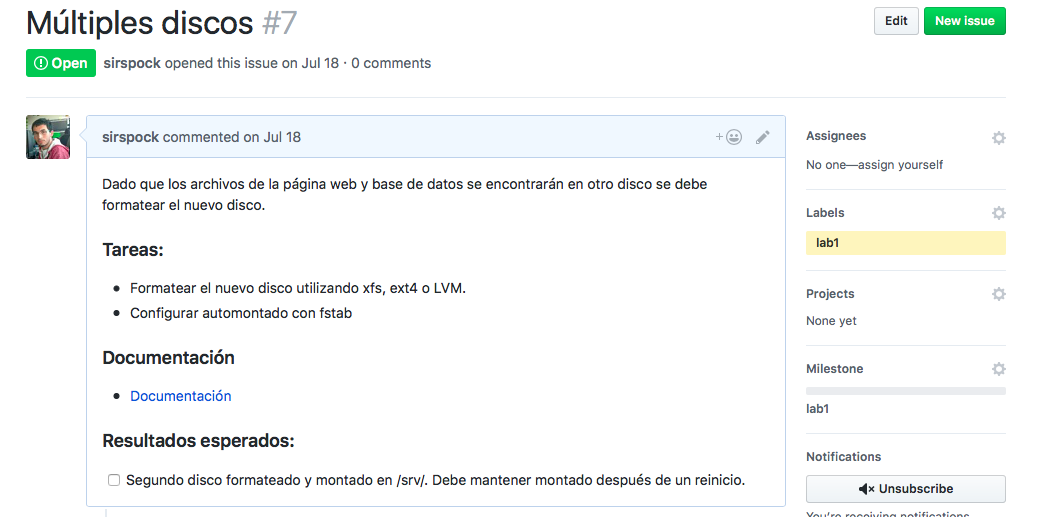
\includegraphics[width=\textwidth,height=1\textheight,keepaspectratio]{images/ej}
\end{figure}

\end{frame}
%------------------------------------------------
\begin{frame}[fragile]
\frametitle{Uso de Github para el curso}
\begin{itemize}
  \item Documentación de los laboratorios se escribe en la wiki de Github. Consejo: documente no solo afectará en la evaluación sino en los siguientes labs.
  \item En los issues, usted puede comentar si tiene problemas.
\end{itemize}

\end{frame}
%------------------------------------------------


\end{document}